\section*{Exercise 3.1}
\enum{
\item
We know that
\spl{
    &P[\text{a random sample of 50 pages contains at least one error}]\\
    =&1-P[\text{a random sample of 50 pages contains no error}]\\
    =&1-(\frac{150}{200})^5\\
    \approx&0.763.
}
\item
We denote that the probability of being sampled is $p$, then
\spl{
    &P[\text{a random sample of 50 pages contains at least three error}]\\
    =&\sum_{k=3}^5\binom{5}{k}p^k(1-p)^{5-k}\\
    \approx&1-\Phi(\frac{3-1/2-5p}{\sqrt{5p(1-p)}})\\
    \overset{!}{=}&90\%.
}

Thus
\spl{
    &\frac{3-1/2-5p}{\sqrt{5p(1-p)}}=-1.29,\\
    &p=0.750.\\
    &n=200p\approx150.
}
Hence, the random sample must contain 150 pages.
} 

\section*{Exercise 3.2}
\enum{
\item
\spl{
R_1(t)&=1-\int_0^t 0.003x^{-0.5}e^{-0.006x^{0.5}}\dd x=1-(-e^{-0.006x^{0.5}})\bigg|_0^t=e^{-0.006t^{0.5}}.\\
R_2(t)&=1-\int_0^t\frac{1}{25000}e^{-\frac{x}{25000}}=1-(-e^{-\frac{x}{25000}}\bigg|_0^t)=e^{-t/25000}.\\
R_s(t)&=\prod_{i=1}^2R_1(t)R_2(t)=e^{-0.006t^{0.5}-t/25000}.
}

Hence, at 2500 hours,
\spl{
    R_s(2500)\approx0.67.
}

\item
\spl{
    F_s(t)=1-R_s(t)=1-e^{-0.006t^{0.5}-t/25000}.
}

When $t<2000$, the probability that the system fails is
\spl{
    F_s(2000)=0.29.
}

\item
\spl{
    &R_p(t)=1-\prod_{i=1}^2(1-R_1(t))(1-R_2(t))\\
    =&R_1(t)+R_2(t)-R_1(t)R_2(t)\\
    =&e^{-0.006t^{0.5}}+e^{-t/25000}-e^{-0.006t^{0.5}-t/25000}.
}
Hence, at 2500 hours,
\spl{
    R_p(t)\approx0.98.
}
}

\section*{Exercise 3.3}
\enum{
\item
\spl{
    \sum_{x=1}^n\sum_{y=x}^n f_{XY}(x,y)=\sum_{x=1}^n\sum_{y=x}^n\frac{2}{n(n+1)}=\frac{n(n+1)}{2}\frac{2}{n(n+1)}=1.
}
Also, $f_{XY}(x,y)>=0$.
Hence, $f_{XY}(x,y)$ is a density.

\item
To find the marginal density,
\spl{
    &f_X(x)=\sum_{y=x}^n\frac{2}{n(n+1)}=\frac{2(n-x+1)}{n(n+1)}.\\
    &f_Y(y)=\sum_{x=1}^y\frac{2}{n(n+1)}=\frac{2y}{n(n+1)}.\\
}

\item
\spl{
    f_X(x)f_Y(y)&=\frac{2(n-x+1)}{n(n+1)}\frac{2y}{n(n+1)}\\
    &=\frac{4y(n-x+1)}{n^2(n+1)^2}\neq\frac{2}{n(n+1)}.
}

Thus, $X$ and $Y$ are not independent.

\item
\spl{
    P[X\leq 3 \text{ and } Y\leq 2]=\sum_{x=1}^3\sum_{y=x}^2\frac{2}{5\cdot(5+1)}=\frac{1}{15}\times3=\frac{1}{5}.
}
}

\section*{Exercise 3.4}
We denote that $V=Y$. Considering $(x,y)\to(u,v)$, we apply
\spl{
    f_{U,V}(u,v)=f_{X,Y}\circ H^{-1}(u,v)\cdot|\text{det} DH^{-1}(u,v)|,
}
where $(x,y)=H^{-1}(u,v)=(u-v,v)$ and det $DH^{-1}(u,v)=1$.

Thus,
\spl{
    f_{U,V}(u,v)=f_{XY}(u-v,v).
}

Hence, the marginal density is
\spl{
    f_U(u)=\int_{-\infty}^{\infty}f_{XY}(u-v,v)dv.
}

\section*{Exercise 3.5}
We know that
\[
    f_X(x)=
    \left\{
    \begin{aligned}
        &\frac{1}{3}e^{-\frac{x}{3}}, \quad x>0\\
        &0, \quad x\leq0\\
    \end{aligned}
    \right.
    ,
    \quad
    f_Y(y)=
    \left\{
    \begin{aligned}
        &e^{-y}, \quad y>0\\
        &0, \quad y\leq0\\
    \end{aligned}
    \right.
\]

Since $U=X+Y$, then
\spl{
    f_U(u)&=\int_0^{u}\frac{1}{3}e^{-\frac{x}{3}}e^{-(u-x)}\dd x\\
    &=\frac{1}{3}e^{-u}\int_0^ue^{\frac{2}{3}x}\dd x\\
    &=\frac{1}{2}e^{-u}(e^{\frac{2}{3}u}-1)\\
    &=(e^{-u/3}-e^{-u})/2.
}

\section*{Exercise 3.6}
We assume that $X_1$ and $X_2$ are independent. Otherwise we cannot determine their covariance.
We know that
\spl{
    f_1(x)&=\frac{1}{\sqrt{2\pi}\sigma_1}e^{-\frac{(x-\mu_1)^2}{2\sigma_1^2}}\\
    m_1(t)&=e^{\mu_1 t+\sigma_1^2t^2/2}\\
    f_2(x)&=\frac{1}{\sqrt{2\pi}\sigma_2}e^{-\frac{(x-\mu_2)^2}{2\sigma_2^2}}\\
    m_2(t)&=e^{\mu_2 t+\sigma_2^2t^2/2}\\
}

First we prove that if $Z=\alpha X$, then $m_Z(t)=m_X(\alpha t)$.

\spl{
    &m_Z(t)=E[e^{tZ}]= E[e^{\alpha tX}]\\
    &=E[e^{(\alpha t)X}]\\
    &=m_X(\alpha t).
}

Also, we know that if $Z=X+Y$, then $m_Z(t)=m_X(t)m_Y(t)$.

Since $Y=\lambda_1X_1+\lambda_2X_2$, then
\spl{
    m_Y(t)=&m_{X_1}(\lambda_1 t)m_{X_2}(\lambda_2 t)\\
    &=e^{\mu_1 \lambda_1t+\sigma_1^2(\lambda_1t)^2/2+\mu_2 \lambda_2t+\sigma_2^2(\lambda_2t)^2/2}\\
    &=e^{(\mu_1\lambda_1+\mu_2\lambda_2)t+(\sigma_1^2\lambda_1^2+\sigma_2^2\lambda_2^2)t^2/2}.
}

Hence, $Y$ follows normal distribution, where
\spl{
    E[Y]&=\lambda_1\mu_2+\lambda_2\mu_2,\\
    \text{Var} Y&=\sigma_1^2\lambda_1^2+\sigma_2^2\lambda_2^2.\\
}

\section*{Exercise 3.7}
\enum{
\item
\spl{
    f_{X_1}(x_1)&=\int_{-\infty}^\infty f_{X_1X_2}(x_1,x_2)\dd x_2\\
    &=\frac{1}{2\pi\sigma_1\sigma_2\sqrt{1-\varrho^2}}\int_{-\infty}^\infty e^{-\frac{1}{2(1-\varrho^2)}[(\frac{x_1-\mu_1}{\sigma_1})^2-2\varrho(\frac{x_1-\mu_1}{\sigma_1})(\frac{x_2-\mu_2}{\sigma_2})+(\frac{x_2-\mu_2}{\sigma_2})^2]}\dd x_2\\
}

Since
\spl{
    -2\varrho(\frac{x_1-\mu_1}{\sigma_1})(\frac{x_2-\mu_2}{\sigma_2})+(\frac{x_2-\mu_2}{\sigma_2})^2=(\frac{x_2-\mu_2}{\sigma_2}-\varrho(\frac{x_1-\mu_1}{\sigma_1}))^2-\varrho^2(\frac{x_1-\mu_1}{\sigma_1})^2,
}
then
\spl{
    f_{X_1}(x_1)=\frac{1}{2\pi\sigma_1\sigma_2\sqrt{1-\varrho^2}}e^{-\frac{(x_1-\mu_1)^2}{2\sigma_1^2}}\int_{-\infty}^\infty e^{-\frac{1}{2(1-\varrho^2)}(\frac{x_2-\mu_2}{\sigma_2}-\varrho(\frac{x_1-\mu_1}{\sigma_1}))^2}\dd x_2.
}

We denote that
\spl{
    t=-\frac{1}{\sqrt{1-\varrho^2}}(\frac{x_2-\mu_2}{\sigma_2}-\varrho(\frac{x_1-\mu_1}{\sigma_1})).
}

Hence,
\spl{
    f_{X_1}(x_1)&=\frac{1}{2\pi\sigma_1}e^{-\frac{(x_1-\mu_1)^2}{2\sigma_1^2}}\int_{-\infty}^\infty e^{-\frac{t^2}{2}}\dd t\\
    &=\frac{1}{\sqrt{2\pi}\sigma_1}e^{-\frac{(x_1-\mu_1)^2}{2\sigma_1^2}}.
}

Hence $x_1\sim N(\mu_1,\sigma_1^2)$.
\item
We know that the coefficient of correlation of $X_1$ and $X_2$ is
\spl{
    \varrho_{X_1X_2}&=\frac{\text{Cov}(X_1,X_2)}{\sigma_1\sigma_2}=\frac{E[(X_1-\mu_1)(X_2-\mu_2)]}{\sigma_1\sigma_2}\\
    &=\frac{\iint_{\mathbb{R}^2}(x_1-\mu_1)(x_1-\mu_2)f_{X_1X_2}(x_1,x_2)\dd x_1\dd x_2}{\sigma_1\sigma_2}
}

We denote $u=\frac{x_1-\mu_1}{\sigma_1}$ and $v=\frac{x_1-\mu_2}{\sigma_2}$, then
\spl{
    &\iint_{\mathbb{R}^2}(x_1-\mu_1)(x_2-\mu_2)f_{X_1X_2}(x_1,x_2)\dd x_1\dd x_2\\
    =&\frac{\sigma_1\sigma_2}{2\pi\sqrt{1-\varrho^2}}\int_{-\infty}^{\infty}\int_{-\infty}^{\infty}uv \exp\bigg[-\frac{1}{2(1-\varrho^2)}(u^2-2\varrho uv+v^2)\bigg]\dd u\dd v\\
    &=\frac{\sigma_1\sigma_2}{2\pi\sqrt{1-\varrho^2}}\int_{-\infty}^{\infty}\int_{-\infty}^{\infty}uv\exp\bigg[-\frac{u^2}{2}-\frac{(v-\varrho u)^2}{2(1-\varrho^2)}\bigg]\dd u\dd v\\
    &=\frac{\sigma_1\sigma_2}{2\pi\sqrt{1-\varrho^2}}\int_{-\infty}^{\infty}ue^{-\frac{u^2}{2}}\bigg[\int_{-\infty}^{\infty}v e^{-\frac{(v-\varrho u)^2}{2(1-\varrho^2)}}\dd v\bigg]\dd u\\
    &=\sigma_1\sigma_2\int_{-\infty}^{\infty}\frac{u}{\sqrt{2\pi}}e^{-\frac{u^2}{2}}\bigg[\int_{-\infty}^{\infty}\frac{v}{\sqrt{2\pi}\sqrt{1-\varrho^2}}e^{-\frac{(v-\varrho u)^2}{2(1-\varrho^2)}}\dd v\bigg]\dd u\\
    &=\sigma_1\sigma_2\int_{-\infty}^{\infty}\frac{u}{\sqrt{2\pi}}e^{-\frac{u^2}{2}}\cdot \varrho u\ \dd u\\
    &=\varrho\sigma_1\sigma_2\int_{-\infty}^{\infty}\frac{u^2}{\sqrt{2\pi}}e^{-\frac{u^2}{2}}\dd u\\
    &=\varrho\sigma_1\sigma_2.
}

Hence,
\spl{
    \varrho_{X_1X_2}=\frac{\varrho\sigma_1\sigma_2}{\sigma_1\sigma_2}=\varrho.
}

\item
Sufficiency:

if $\varrho=0$, then 
\spl{
    f_{X_1X_2}(x_1,x_2)=\frac{1}{2\pi\sigma_1\sigma_2}e^{-\frac{1}{2}[(\frac{x_1-\mu_1}{\sigma_1})^2+(\frac{x_2-\mu_2}{\sigma_2})^2]}.
}
Also,
\spl{
    f_{X_1}(x_1)f_{X_2}(x_2)&=\frac{1}{2\pi\sigma_1\sigma_2}e^{[-(\frac{x_1-\mu_1}{2\sigma_1}^2+\frac{x_2-\mu_2}{2\sigma_2})^2]}\\
    &=f_{X_1X_2}(x_1,x_2),
}
which means $X_1$ and $X_2$ are independent.

Necessity:

if $X_1$ and $X_2$ are independent, then
\spl{
    f_{X_1X_2}(x_1,x_2)=f_{X_1}(x_1)f_{X_2}(x_2).
}
Specially, when $x_1=\mu_1$ and $x_2=\mu_2$,
\spl{
    \frac{1}{2\pi\sigma_1\sigma_2\sqrt{1-\varrho^2}}=\frac{1}{\sqrt{2\pi}\sigma_1\sqrt{2\pi}\sigma_2}.
}

Hence $\varrho=0$.

It's not true for a bivariate random variable with an arbitrary distribution. 

For example,
\begin{table}[H]
    \centering
    \begin{tabular}{c|cccc}
        X,Y & 0 & $\frac{1}{4}$ & 1\\\hline
        -1 & 0 & 0 & $\frac{1}{5}$\\
        $\frac{1}{2}$ & 0 & $\frac{1}{5}$ & 0\\
        0 & $\frac{1}{5}$ & 0 & 0\\
        $\frac{1}{2}$ & 0 & $\frac{1}{5}$ & 0\\        
        1 & 0 & 0 & $\frac{1}{5}$\\        
    \end{tabular}
\end{table}

Here we know that $Y=X^2$. However,
\spl{
    &E[XY]=-\frac{1}{5}+\frac{1}{8}\frac{1}{5}+0\frac{1}{5}+\frac{1}{5}-\frac{1}{8}\frac{1}{5}=0,\\
    &E[X]E[Y]=0,\quad E[Y]=0.\\
    &\text{Cov}(X,Y)=E[XY]-E[X]E[Y]=0.
}

Here $\varrho_{XY}=0$, but $X$ and $Y$ are not independent.

\item
First, we derive the conditional density
\spl{
    f_{X_2|_{x_1}}=\frac{f_{X_1X_2}(x_1,x_2)}{f_{X_1}(x_1)}.
}
Then, we denote $u=\frac{x_1-\mu_1}{\sigma_1}$ and $v=\frac{x_1-\mu_2}{\sigma_2}$.

\spl{
    \mu_{X_2|_{x_1}}&=E[X_2|_{x_1}]=\int_{-\infty}^\infty x_2f_{X_2|_{x_1}}(x_2)\dd x_2\\
    &=\sigma_2\int_{-\infty}^\infty \frac{v\sigma_2+\mu_2}{\sqrt{2\pi}\sigma_2\sqrt{1-\varrho^2}}e^{-\frac{1}{2(1-\varrho^2)(u^2-2\varrho uv+v^2)}}e^{-\frac{u^2}{2}}\dd v\\
    &=\int_{-\infty}^\infty \frac{v\sigma_2+\mu_2}{\sqrt{2\pi}\sqrt{1-\varrho^2}}e^{-\frac{u^2}{2}-\frac{(v-\varrho u)^2}{2(1-\varrho^2)}}e^{\frac{u^2}{2}}\dd u\\
    &=\int_{-\infty}^\infty \frac{v\sigma_2+\mu_2}{\sqrt{2\pi}\sqrt{1-\varrho^2}}e^{-\frac{(v-\varrho u)^2}{2(1-\varrho^2)}}\dd u\\
    &=\sigma_2\int_{-\infty}^\infty \frac{v}{\sqrt{2\pi}\sqrt{1-\varrho^2}}e^{-\frac{(v-\varrho u)^2}{2(1-\varrho^2)}}\dd u+\mu_2\int_{-\infty}^\infty \frac{1}{\sqrt{2\pi}\sqrt{1-\varrho^2}}e^{-\frac{(v-\varrho u)^2}{2(1-\varrho^2)}}\dd u\\
    &=\sigma_2\varrho u+\mu_2\\
    &=\mu_2+\varrho\frac{\sigma_2}{\sigma_1}(x_1-\mu_1).
}
}

\section*{Exercise 3.8}
\enum{
\item
unit:10.

\begin{table}[H]
    \centering
    \begin{tabular}{c|l}
        Stem & Leaves\\\hline
        532 & 9 \\
        534 & 2 \\
        535 & 47 \\
        536 & 6 \\
        537 & 5678 \\
        538 & 12345778888 \\
        539 & 016999 \\
        540 & 11166677889 \\
        541 & 123666688 \\
        542 & 0011222357899 \\
        543 & 01111556 \\
        544 & 00012455678 \\
        545 & 233447899 \\
        546 & 23569 \\
        547 & 357 \\
        548 & 11257 \\
    \end{tabular}
\end{table}

We can approximately conclude that it follows a shape of normal distribution.

\item
We know that n=100, so that the number of categories is 8.

The data range is 5487-5329=158. The category length is $\lceil{158/8}\rceil=20$.

The lower bound is $5329-0.5=5328.5$.

{
\ttfamily Histogram[Data, {Min[cat], Max[cat], 20}, PlotRange -> {0, Automatic},\\
Frame -> {True, True, False, False}, \\
FrameTicks -> {{Automatic, None}, {cat, None}}, \\
FrameLabel -> {"Shear strength of spot welds", "Number of welds"}]
}

\begin{figure}[H]
    \centering
    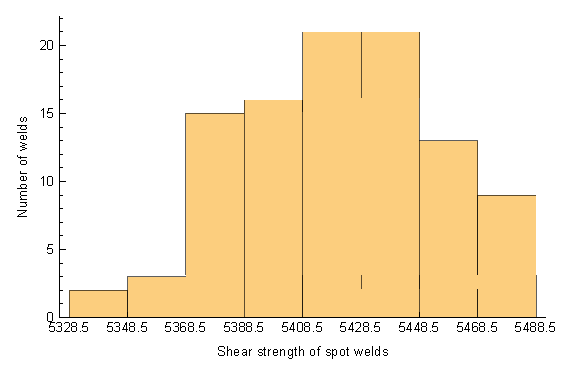
\includegraphics[height=6.5cm]{images/382}
    \caption{Shear strength distribution of 100 sample welds}
\end{figure}

The histogram obtains a shape similar to normal distribution, conveying the same information as the stem-leaf display.

\item
\spl{
    &q_1=5399\quad q_2=5421.2\quad q_3=5445.5.\\
    &iqr=46.5,\quad f_1=5329.25,\quad f_3=5515.25.\\
    &a_1=5342,\quad a_3=5487.
}
\begin{figure}[H]
    \centering
    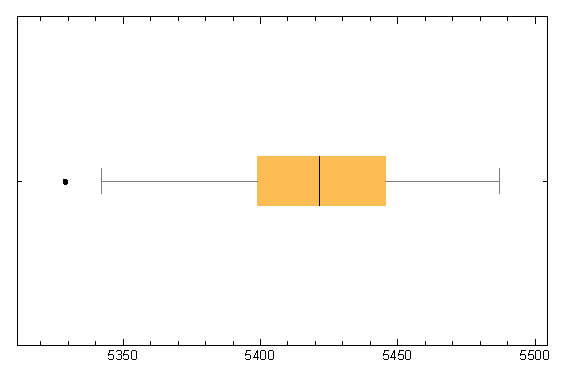
\includegraphics[height=6.5cm]{images/383}
    \caption{Boxplot of shear strength of 100 sample welds}
\end{figure}

Boxplot demonstrates the distribution more simply and clearly, stating the key points without specific data values. Stem and leaf diagram is more complicated but keeps all the details.
}

\section*{Exercise 3.9}
\enum{
\item
unit:1.
\begin{table}[h]
    \centering
    \begin{tabular}{c|l}
        Stem & Leaves\\\hline
        10&1\\
        22 & 588\\
        23 & 02234\\
        23 & 558\\
        24 & 023\\
    \end{tabular}
\end{table}
\item
Sample mean: 22.16.

Sample median: 23.35.

Sample standard deviation: 3.47.

\item
\begin{figure}[H]
    \centering
    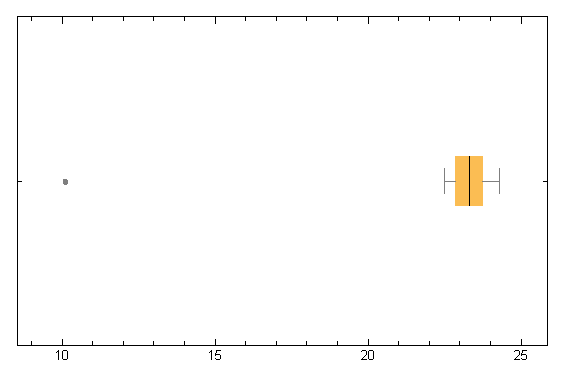
\includegraphics[height=6.5cm]{images/393}
    \caption{Boxplot of temperature samples}
\end{figure}

\item
Sample mean: 23.39.

Sample median: 23.35.

Sample standard deviation: 0.54.

The sample mean is more accurate after we drop the outlier. The sample standard deviation is much less than before because the degree of dispersion is less.
}

\section*{Exercise 3.10}
\spl{
    L(\gamma)&=\prod_{i=1}^nf(X_i)=\prod_{i=1}^n(\gamma+1)x_i^\gamma\\
    &=(\gamma+1)^n(\prod_{i=1}^n x_i)^\gamma.
}

We take the logarithm,
\spl{
    \ln L(\gamma)&=n\ln (\gamma+1)+\gamma\ln (\prod_{i=1}^n x_i)\\
    &=n\ln (\gamma+1)+\gamma\sum_{i=1}^n \ln(x_i).
}

Thus,
\spl{
    \frac{\dd}{\dd \gamma}L(\gamma)&=\frac{n}{\gamma+1}+\sum_{i=1}^n \ln(x_i)=0.\\
    \gamma&=-\frac{1}{n\sum_{i=1}^n \ln(x_i)}-1.
}

\section*{Exercise 3.11}
\enum{
\item
We know that the density function is
\spl{
    f(x)=\binom{4}{x}p^x(1-p)^{4-x}, \quad x=0,1,2,3,4.
}

Thus,
\spl{
    L(p)=\bigg[\binom{4}{0}p^0(1-p)^4\bigg]^8\bigg[\binom{4}{1}p^1(1-p)^3\bigg]^6\bigg[\binom{4}{2}p^2(1-p)^2\bigg]=24p^8(1-p)^{52}.
}

We take the derivative,
\spl{
    \frac{\dd}{\dd p}L(p)&=24(8p^7(1-p)^{52}-p^8\cdot52(1-p)^51)=0,\\
    p&=\frac{2}{15}.
}

\item
The expectation of failed brake shoes is
\spl{
    E[X]=np=4\cdot\frac{2}{15}=\frac{8}{15}.
}

Hence the failure rate is
\spl{
    p=\frac{E[X]}{n}=\frac{2}{15}\approx0.133>0.1.
}

Hence, I will have some doubts concerning the use of this new material.
}